\section{Ejes de estudio}

Los ejes de estudio en los que nos centraremos son:
\begin{itemize}
    \item ¿Cómo varían las cancelaciones y retrasos por clima a través del tiempo? ¿Cómo influye el aeropuerto de origen?
    \item ¿Cómo se comporta nuestro modelo de cuadrados mínimos con diferentes aerolineas? ¿Podemos predecir alguna mejor que otra?
\end{itemize}

\todo[inline]{REVISAR SI ES QUE REALMENTE HICIMOS ESTO QUE DICE}

En el primer eje trataremos de encontrar un patrón a las cancelaciones por clima a través del tiempo. ¿Se sigue un patrón regular?, ¿Hay fechas en las cuáles siempre hay cancelaciones? Veremos además que sucede con los retrasos en algunos aeropuertos particulares. \\

En el segundo eje analizaremos las aerolíneas. Nos centraremos en algunas más representativas y veremos las regularidades (o irregularidades) que poseen. ¿Hay alguna más dificil de predecir que otras? ¿Cómo se comporta una misma familia de funciones de cuadrados mínimos con distintas aerolineas? ¿Será necesario adaptarlo cada vez? \\

\section{Desarrollo}



\section{Cancelaciones por clima}

\subsection{Preliminares}

En esta sección veremos cómo varían las cancelaciones por clima a través del tiempo, y veremos si podemos encontrar algún patrón. Nos será muy util contar con los motivos de las cancelaciones para poder diferenciar las que nos interesa, pero sin embargo, los datos previos a 2003 no cuentan con esta información. Es por eso que tomaremos los datos desde 2003 en adelante. \\

Con respecto a los gráficos que mostraremos, en un principio agrupamos los datos por mes pero con ello perdíamos información: hay valores que varían semana a semana dentro de un mismo mes. Por ello decidimos agrupar nuestros datos por semanas. \\

Sobre los retrasos, consideraremos que un vuelo tiene retraso cuando su tiempo de demora es superior a los 15 minutos. Esto se corresponde con la métrica de \textit{On Time Performance} (OTP) propuesta en el enunciado del trabajo. \\

\subsection{Experimentación}

En primer lugar tomaremos las cancelaciones por climas de manera general. Esperamos que haya una regularidad periódica, dónde para un mismo mes en diferentes años se registren cancelaciones comparables, pues tenemos en mente que hay épocas marcadas con tormentas fuertes o huracanes. \\

{\centering
    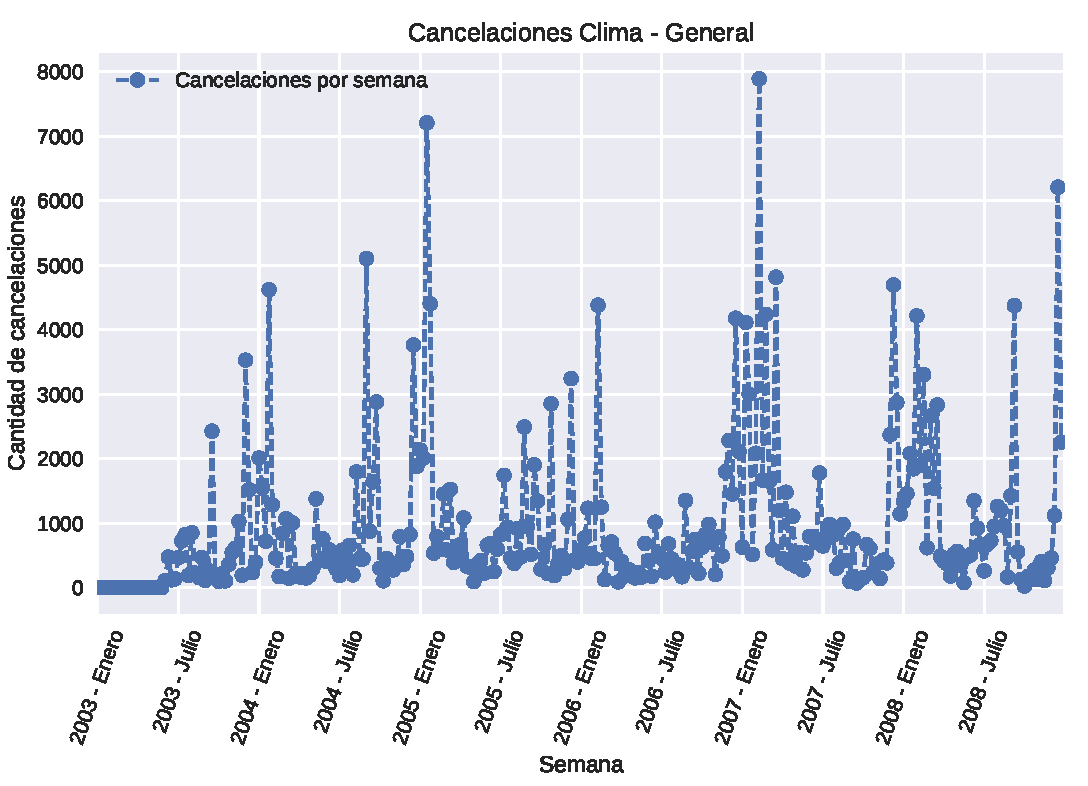
\includegraphics[scale=0.8]{informe/imagenes/cancelacionesClimaGeneralPlotV1.pdf} \\
    \captionof{figure}{Cancelaciones por clima con respecto al tiempo.\\}
}
$ $\newline

Analicemos un poco los datos. El comienzo de 2003 se ve completamente en cero, esto es por la falta de datos sobre cancelaciones climáticas en ese período. En las estimaciones de cuadrados mínimos no tendremos en cuenta este período sin datos, por lo que no nos será de ningún problema. \\

En enero y diciembre (invierno de USA) siempre se observan mayor cantidad de cancelaciones. Consideramos que esto puede deberse a dos motivos: Tormentas de nieve y mal clima en general, y el aumento del caudal de gente que viaja en épocas festivas. \\




% @Jonno:  Se puede quitar, me parecio piola como comentario de que averiguamos cosas.
Como curiosidad, en agosto de 2003 se encuentra un pico aislado de los demás. Coincide con un apagón en grandes ciudades (Por ej, Nueva York) que duró 24hs en el cuál se reportaron cancelaciones de vuelos. Si bien uno creería que no tiene por qué estar relacionado al clima, el apagón se produjo por una caída del servicio central por las grandes demandas debido a las temperaturas inusuales de hasta 40 grados. \cite{ApagonNewYork}\\


% Pico aislado en Agosto de 2003
% http://www.elmundo.es/elmundo/2003/08/14/internacional/1060893592.html

% Agosto 2004: Charley
% https://es.wikipedia.org/wiki/Hurac%C3%A1n_Charley_(2004)

% Agosto 2005: Katrina
% https://es.wikipedia.org/wiki/Hurac%C3%A1n_Katrina


